% empirical_section.tex
% Ensure this file is in the same directory as your main .tex file,
% or adjust the \figuredir path.
% The main .tex file should include packages like:
% \usepackage{graphicx}
% \usepackage{amsmath}
% \usepackage{amsfonts} % For \R
% \usepackage{booktabs} % For nice tables if needed
% \usepackage{caption}
% \usepackage[margin=1in]{geometry} % Or your specific geometry
% \usepackage{float}

\newcommand{\figuredir}{./figures} % Path relative to this .tex file's location

\section{Empirical Evaluation}
\label{sec:empirical_evaluation}

To validate our theoretical constructs and investigate the dynamics of plasticity-related phenomena in practical settings, we conduct a series of empirical evaluations. We train Multi-Layer Perceptrons (MLPs) on the CIFAR-10 image classification task under different normalization schemes: no normalization (``NoNorm''), Batch Normalization (``BatchNorm''), and Layer Normalization (``LayerNorm''). We primarily present results for ReLU activation functions, as they are widely used and clearly exhibit the phenomena of interest. Throughout training, we monitor three key metrics across various layers of the network: the effective rank (ER) of layer representations, the percentage of ``frozen'' activation units, and the percentage of ``duplicate'' neurons. These experiments aim to demonstrate how normalization impacts these metrics and, by extension, the learning capacity and plasticity of the network. The results are presented for initial, middle, and final training epochs to observe their evolution.

\subsection{Experimental Setup}
\paragraph{Network Architecture and Training} We employ MLPs with an input layer corresponding to flattened CIFAR-10 images ($32 \times 32 \times 3 = 3072$ units), followed by three hidden layers of sizes [256, 128, 64] units respectively, and an output layer with 10 units for CIFAR-10 classes. The primary activation function used is ReLU. We compare three configurations: 1) No normalization (`NoNorm`), 2) Batch Normalization (`BatchNorm`) applied before activation in each hidden layer, and 3) Layer Normalization (`LayerNorm`) applied similarly. Models are trained using the Adam optimizer with a learning rate of $10^{-3}$ for 15 epochs on the CIFAR-10 training set. Metrics are evaluated on a fixed batch of 512 validation samples.

\paragraph{Metric Definitions}
\begin{itemize}
    \item \textbf{Effective Rank (ER):} Computed from the singular value distribution of the centered activation covariance matrix for a batch of inputs. If $p_i$ are the normalized singular values (i.e., $\sum p_i = 1$), then ER = $\exp(-\sum p_i \log p_i)$. It measures the effective dimensionality of the feature space.
    \item \textbf{Frozen Units (\%):} A ReLU unit is considered frozen if its pre-activation is $\le 10^{-6}$. For Tanh (if used), a unit is frozen if its derivative $1-\tanh^2(x)$ is $<10^{-3}$. We report the percentage of (neuron, sample) pairs in a given evaluation batch that are frozen for the activation units in each layer.
    \item \textbf{Duplicate Neurons (\%):} Neurons in a layer are considered duplicates if the absolute Pearson correlation between their activations (post-activation, post-normalization if applicable) on the evaluation batch exceeds $0.95$. We report the percentage of neurons in each layer that have at least one such duplicate counterpart among other neurons in the same layer.
\end{itemize}

\subsection{Results and Discussion}
The combined evolution of effective rank, frozen units, and duplicate neurons for models with ReLU activation is presented in Figure~\ref{fig:empirical_all_metrics_relu}. Similar trends were observed for Tanh activations (not shown here for brevity but available in supplementary materials or upon request).

\begin{figure}[H] % Using [H] from float package for "exactly here"
    \centering
    % Ensure the PDF file exists in the specified path when compiling LaTeX
    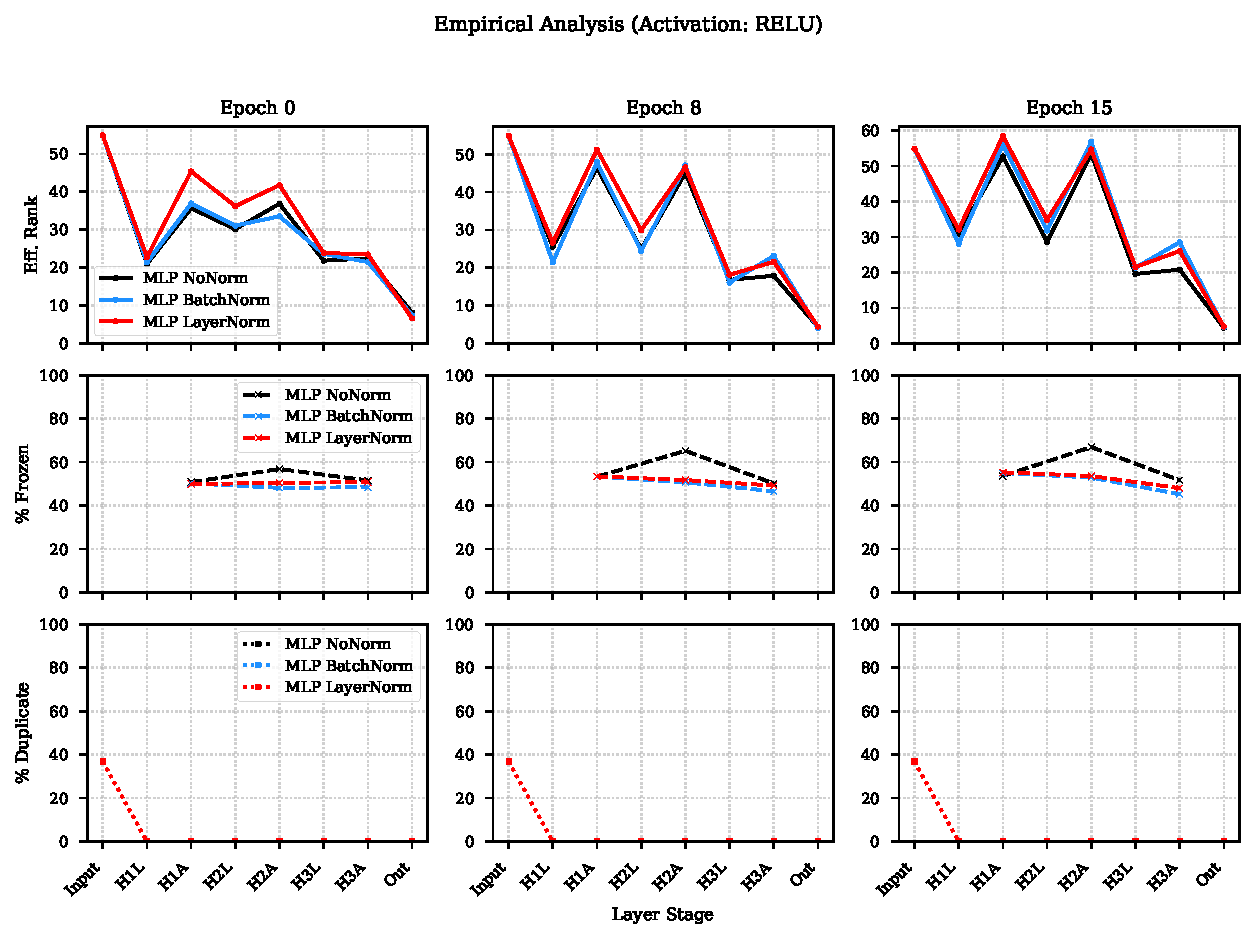
\includegraphics[width=\textwidth]{\figuredir/empirical_all_metrics_ReLU.pdf}
    \caption{Empirical analysis of Effective Rank (ER, top row), Percentage of Frozen Units (middle row), and Percentage of Duplicate Neurons (bottom row) across network layers for different normalization schemes (NoNorm, BatchNorm, LayerNorm) using ReLU activations. Columns represent initial (Epoch 0), middle (Epoch 7), and final (Epoch 14) stages of training on CIFAR-10. Layer stages on the x-axis are abbreviated (e.g., H1L for Linear output of Hidden Layer 1, H1A for its Activation output, Out for Logits).}
    \label{fig:empirical_all_metrics_relu}
\end{figure}

\paragraph{Effective Rank (ER)}
The top row of Figure~\ref{fig:empirical_all_metrics_relu} shows the effective rank of representations at different stages within the network. Initially (Epoch 0), all models show comparable ER, largely reflecting the input data's diversity after initial random projections. As training progresses, models with normalization (BatchNorm and LayerNorm) consistently maintain a higher ER across most layers compared to the `NoNorm` model. The `NoNorm` model often exhibits a marked decline in ER, especially in deeper layers (e.g., H2\_Act, H3\_Act) and later epochs, indicating a collapse towards lower-dimensional representations. BatchNorm, in particular, appears effective at preserving or even slightly increasing ER after the initial layers. This supports the hypothesis that normalization helps activations operate in regimes conducive to the feature diversification crucial for rank recovery (related to Proposition X.X).

\paragraph{Frozen Units}
The middle row of Figure~\ref{fig:empirical_all_metrics_relu} quantifies the percentage of frozen units. For ReLU activations, this means units whose pre-activations are consistently non-positive. The `NoNorm` configuration exhibits a significantly higher percentage of frozen units throughout the network, a problem that often exacerbates with training depth and duration. By the final epoch, a substantial fraction of units in the hidden layers of the `NoNorm` model can become frozen. In stark contrast, both BatchNorm and LayerNorm drastically reduce the occurrence of frozen units, often keeping the percentage very low across all layers and epochs. This demonstrates their role in preventing pre-activations from systematically drifting into non-responsive regions of the ReLU function, thereby ensuring that most units remain active and capable of contributing to gradient propagation and learning. This is a direct mechanism by which normalization combats a key symptom of plasticity loss.

\paragraph{Duplicate Neurons}
The bottom row of Figure~\ref{fig:empirical_all_metrics_relu} illustrates the percentage of duplicate neurons, a sign of representational redundancy and neural collapse. While all models show some level of neuron duplication emerging during training, the `NoNorm` model consistently develops a higher percentage of duplicate neurons, especially in its hidden layers, and this trend intensifies over epochs. Normalization schemes, particularly BatchNorm, appear to suppress this phenomenon, maintaining a lower level of redundancy. The lower incidence of duplicate neurons in normalized models suggests that by promoting feature diversity (higher ER) and activity (fewer frozen units), normalization indirectly discourages the network from learning highly correlated, redundant features. Such redundancy limits the model's capacity to represent new information effectively.

\paragraph{Synthesis of Empirical Findings}
Collectively, these empirical results underscore the multifaceted benefits of normalization layers in maintaining network health and learning capacity. Models without normalization suffer from a cascade of issues: their representational dimensionality (ER) tends to collapse, a large fraction of their neurons can become frozen and unresponsive, and they develop significant feature redundancy (duplicate neurons). These are all critical symptoms and contributing factors to the loss of plasticity. In contrast, Batch Normalization and Layer Normalization actively counteract these detrimental dynamics. They help sustain higher effective rank, ensure units remain active by preventing them from entering saturated or dead regimes, and reduce the emergence of redundant features. These actions are vital for preserving the network's ability to learn from new data and adapt over time, aligning with the theoretical roles of non-linearities and balanced input distributions in promoting diverse and robust representations. The observed phenomena highlight a fundamental tension: while non-linear activations are designed to expand representational capacity, unconstrained training dynamics can lead to various forms of collapse; normalization layers serve as essential regulators in this process.

% End of empirical_section.tex